\section{Good practices in AI/ML and checklists}
\begin{frame}
  \frametitle{Table of Contents}
  \tableofcontents[currentsection]
\end{frame}

%\subsection{checklist for artificial intelligence in medical imaging (CLAIM)}

\subsection{FDA-approved AI-based Medical Devices}

%%%%%%%%%%%%%%%%%%%%%%%%%%%%%%%%%%%%%%%%%%%%%%%%%%%%%%%%
{
\paper{
Benjamens S., Dhunnoo  P. and  Mesk\'o B. The state of artificial intelligence-based FDA-approved medical devices and algorithms: an online database. npj Digit. Med. 3, 118 (2020).
}
\begin{frame}{
FDA-approved AI-based Medical Devices
}{
%(2019-2021) @ KCL
}
      \begin{figure}
        \centering
        \includegraphics[width=1.0\textwidth]{fda-approved-ai-based-med-devs/outputs/drawing-v00}
        % \caption{The sonographer-probe-patient control system}
      \end{figure}
\end{frame}
}







\subsection{Quality Systems and Good Machine Learning Practices (GMLP) by FDA}
%%%%%%%%%%%%%%%%%%%%%%%%%%%%%%%%%%%%%%%%%%%%%%%%%%%%%%%%
{
\paper{
%\url{https://www.fda.gov/files/medical%20devices/published/US-FDA-Artificial-Intelligence-and-Machine-Learning-Discussion-Paper.pdf}
US-FDA-Artificial-Intelligence-and-Machine-Learning-Discussion-Paper
}
\begin{frame}{
Regulatory Framework for Modifications to \\
(AI/ML)-Based Software as a Medical Device (SaMD)
}{
%(2019-2021) @ KCL
}
      \begin{figure}
        \centering
        \includegraphics[width=1.0\textwidth]{goodALMLFDA/outputs/drawing-v00}
        % \caption{The sonographer-probe-patient control system}
      \end{figure}
\end{frame}
}

%%%%%%%%%%%%%%%%%%%%%%%%%%%%%%%%%%%%%%%%%%%%%%%%%%%%%%%%
{
\paper{
Rajpurkar, Pranav, and Matthew P. Lungren. "The Current and Future State of AI Interpretation of Medical Images." New England Journal of Medicine 388, no. 21 (2023): 1981-1990.
}
\begin{frame}{
Checks for AI Systems in Radiology
}{
%(2019-2021) @ KCL
}
      \begin{figure}
        \centering
        \includegraphics[width=1.0\textwidth]{ai-interpreation-of-medical-images/outputs/drawing-v00}
        % \caption{The sonographer-probe-patient control system}
      \end{figure}
\end{frame}
}



